\documentclass[
 a4paper,twocolumn,showpacs,aip,groupedaddress,%
  eqsecnum,notitlepage,showkeys,cha,longbibliography,10pt
]{revtex4-1}
\usepackage[english]{babel}
\usepackage[utf8x]{inputenc}
\usepackage[T1]{fontenc}
\usepackage{amssymb}
\usepackage{amsmath,latexsym}
\usepackage{graphicx}
\usepackage{dcolumn}
\usepackage{tikz}
\usepackage{natbib}
\usepackage{float}
\usepackage[hyperref]{}
\usepackage[export]{adjustbox}
\usepackage{silence}
\WarningFilter{revtex4-1}{Repair the float}
\usepackage{mathtools}
\usepackage{soul}
\usepackage{array}
\usepackage{tabu}
\usepackage{multirow}
\DeclarePairedDelimiter\bra{\langle}{\rvert}
\DeclarePairedDelimiter\ket{\lvert}{\rangle}
\DeclarePairedDelimiterX\braket[2]{\langle}{\rangle}{#1 \delimsize\vert #2}


\newcommand*{\citen}[1]{%
  \begingroup
    \romannumeral-`\x % remove space at the beginning of \setcitestyle
    \setcitestyle{numbers}%
    \cite{#1}%
  \endgroup   
}

\usepackage[a4paper,top=1.8cm,bottom=1.8cm,left=1.5cm,right=1.5cm]{geometry}
\usepackage[skip=5pt, font=scriptsize, labelfont=bf, justification=raggedright]{caption}

\usepackage{titlesec}

\titlespacing\section{0pt}{12pt plus 4pt minus 2pt}{0pt plus 2pt minus 2pt}

\graphicspath{ {Images/} }

\begin{document}

\title{\LARGE{Free-space Quantum Key Distribution Implementation}}

\author{Lindsey Keary}
\affiliation{ 
Student Number : 17099595, l.keary.17@ucl.ac.uk, University College London
}
\date{\today}

\begin{footnotesize}
\begin{abstract}
The number of photons per pulse is calculated to be $\approx$ 0.6 when operating the diode laser as an approximate single photon source. The < 80 ps laser pulse width cannot be resolved due to the 0.21 ns trigger detection width which provides the ultimate resolution of pulse detection. Despite photon state detection enabling Alice and Bob to remove the bits which are not measured in the incorrect basis, the quantum bit error rate (QBER) for two of the prepared photon states is determined to be too large. The reasons these errors exceed the 15 $\%$ critical error rate which ensures secured transfer of information is therefore investigated.   
\end{abstract} 
\end{footnotesize}

\maketitle
\begin{footnotesize}
\section{\label{sec:level1}Introduction} The aim of cryptography is to provide mathematical tools to keep the contents of private messages indecipherable from a third party observer as the message is being transferred between a source and a receiver \citep{ShenoyHejamadi2017QuantumBeyond}. Cryptography is of importance in sectors such as the ministry of defense and the financial trading market \citep{Diamanti2016PracticalDistribution}. Additionally, the popularity of online payments and banking, including the recent surge in popularly of cryptocurrency, risks personal sensitive data and assets if the security protocols are not in place or become compromised. In 1994 due to the development of quantum algorithms, such as Shor's algorithm and the possibility of building a quantum computer provided evidence that cryptography schemes in the future could become vulnerable to a new type of crytanalysis. The risk to classical cryptography protocols is due the potential for computation of discrete logarithms and factorising integers \citep{ShorAlgorithmsFactoring}. However, the concept of quantum key distribution (QKD) was a very early development in the field of quantum computation, therefore in 1984 the BB84 protocol was theorised \citep{unknown, Bennett2014QuantumTossing}. By 1992 the BB84 scheme was experimentally realised \citep{Bennett1992ExperimentalCryptography}.

The BB84 protocol was the first in a series of devised protocols, discussed in Ref. [\citen{Singh2014QuantumReview}], which rely on the Heisenberg uncertainty to prevent a third party gaining information without being detected. Furthermore, another series of protocols utilised quantum entanglement, with the most famous example being the Erkert protocol \citep{Singh2014QuantumReview}. However, there are several challenges facing the implementation of a large-scale QKD network including; long distance transmission of keys being limited by transmission losses, the requirement for single photon sources and detectors, the need for rapid quantum random generators and protection against attack protocols \citep{Diamanti2016PracticalDistribution,Bedington2017ProgressDistribution}.



   
\begin{figure*}[ht]
\centering
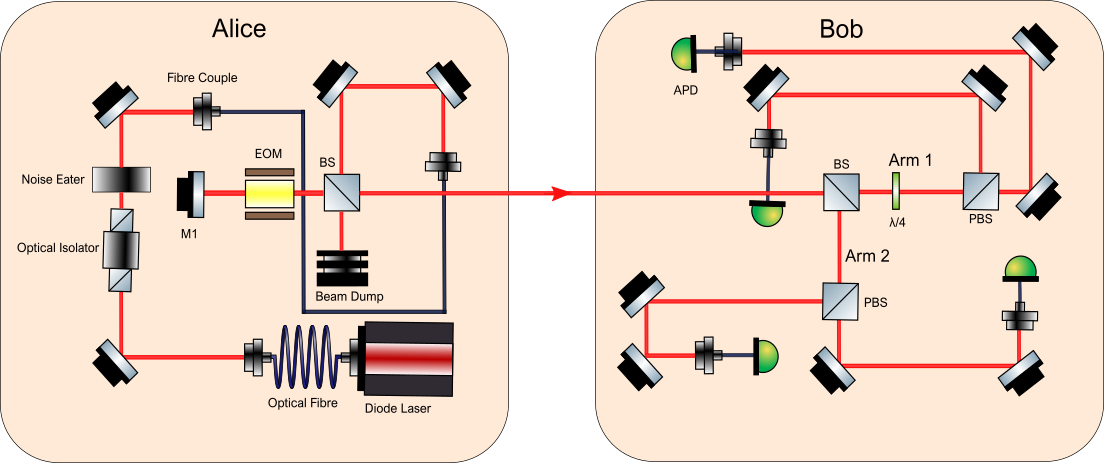
\includegraphics[width=0.7\textwidth,keepaspectratio]{drawing1}
\caption{\label{fig:opticalsetup}The (mostly) free-space BB84 optical set-up. Arm 1 provides detection of the ($\ket{R},\ket{L}$) basis and arm 2 provides detection of the ($\ket{H},\ket{V}$). (Components from the component library created by  Alexander Franzen are used in this figure).}
\end{figure*}
\section{\label{sec:level1}QKD Experimental Implementation}
Quantum cryptography enables a method to share a private key between a source (Alice) and a detector (Bob) while being able to detect the presence of a third-party observer (Eve) who attempts to gain information about the key. The shared key provides a one-time pad which enables Alice to encrypt a message the same length as the key string by adding the corresponding key and message bits together. Bob receives the encrypted message via a public channel and he obtains the message by subtracting the key \citep{Nielsen2010QuantumInformation}.


\subsection{The BB84 protocol}
In the BB84 protocol Alice initially produces a random bit string of length $m$. Alice has the ability to prepare photon states which can be in the horizontally/vertically polarised ($\ket{H}$, $\ket{V}$) basis or right/left-circularly polarised ($\ket{R}$, $\ket{L}$) basis. The states in each basis are allocated as a '0' or '1' bit value eg. $\ket{H}$ = '0' and $\ket{V}$ = '1'. Therefore based on the value of each bit of the randomly generated string, the photon state is chosen randomly between the two polarisation states from different basis which have the correct assigned bit value. Alice sends the $m$ photon states to Bob. Bob randomly decides which basis to measure the prepared states where consequently the states are projected to classical bits. For $\approx$ 50$\%$ of Bob's measurements are the same basis as Alice has prepared the state  and Bob will obtain the correct value of the bit. 50$\%$ of the time Bob's result is completely random. Alice and Bob publicly communicate prepared and measured basis without exposing the values of the bit string or prepared photon states. They retain the bits in which the basis are in agreement. Now the shared key bit string length is reduced to $m/2$ \citep{Fox2006QuantumIntroduction,Bedington2017ProgressDistribution}. 

Following from the no-cloning theorem \citep{Wootters1982ACloned}, Alice and Bob can determine the presence of a third party observer. If Eve captures an encoded photon state, she will make a measurement in a random basis. Thereafter Eve prepares photon in the same basis corresponding to the classical bit result and sends it to Bob. If she guesses the correct basis she gains information of the state and transmits the correct state to Bob. Otherwise there is a 50$\%$ probability of obtaining a random bit value which is correct even when she measures in the incorrect basis. Once the key has been transferred from Alice to Bob, Bob then sends a selection, often $m/4$ of his bits to Alice via the unsecured classical channel. Alice compares her bits to the selection Bob has sent her and then she discards of these bits. The length of the remaining key string is now $m$/4. Under the assumption that the quantum channel is noiseless, if the quantum bit error rate (QBER) is >25$\%$ then Alice can determine that Eve has been eavesdropping and the key is discarded. If the QBER is <25$\%$ the communication of the key is deemed secure \citep{Fox2006QuantumIntroduction,Bedington2017ProgressDistribution}. Error correction is applied to the imperfect key to correct for differences between the key bit strings. This process is known as information reconciliation. Additionally, privacy amplification is used to minimise Eve's knowledge of the distilled key following error-correction \citep{Nielsen2010QuantumInformation}. 


%(\ref{fig:})%
\subsection{Free-space Implementation} 
The set-up must have the capability to produce the four photon states ($\ket{H}$, $\ket{V}$, $\ket{R}$, $\ket{L}$) and have a specific detector assigned for each state. To send the photon states a single photon source is required. The production of single photons is an area of active research, with quantum dot devices currently leading in the race to produce an on demand source of anti-bunched light \citep{Senellart2017High-performanceSources}. The 635 nm diode laser used in this implementation produces a coherent quantum state. Therefore pulsing at <100 MHz and attenuating the power such that the there is a small mean number of photons per pulse, $\bar{N}\approx0.1$, results in $\approx 5\%$ of the pulses containing more than 1 photon \citep{Fox2006QuantumIntroduction}. 

The optical set-up is shown in Fig. (\ref{fig:opticalsetup}) where the light is coupled into the single-mode optical fibre core using an arrangement of focusing lenses. The use of pairs of mirrors increase the degrees of freedom to assist with beam alignment. Initially considering Alice's optical set-up, the optical isolator consists of the Faraday rotator sandwiched between two polarisers. The linearly polarised light is rotated by the applied magnetic flux density of the Faraday rotator such that light is transmitted but cannot be reflected back to the laser source \citep{Saleh2007FundamentalsPhotonics}. The noise eater contains a proportional-differential-integral controller circuit which stabilises the laser intensity. Electro-Optic Modulator (EOM) produces an electronically controlled variable waveplate due to the change in the refractive index, $n$, of the anisotropic crystal in the presence of an applied electric field, $E$. The light undergoes a phase shift given by:

\begin{equation}
\label{eq:interactionham0}
\Delta\phi = -\pi \frac{\chi n^{3}EL}{\lambda },
\end{equation}

where $\lambda$ is the laser wavelength, $L$ is the crystal length and $\chi$ is the electric susceptibility. The distance, $d$ separates the contacts of the voltage applied on different faces of the crystal. To apply a phase shift of $\pi$, a voltage $V_{\pi}=(d\lambda)/(L\chi n^{3})$ is required \citep{Saleh2007FundamentalsPhotonics,Iizuka2002ElementsMedia}. To prepare all four polarisation states the required voltage range is $-V_{\pi}$ to $+V_{\pi}$. 

The voltage signals applied to implement the QKD scheme when used in practice to encode private messages should be generated using a random number generator. However the photon states for this experiment are generated using computational control of a signal generator to produce a repeating sequence of small voltage signals which are sent to the amplifier. Therefore considering that the incoming light is always in the $\ket{V}$ state and for an amplifier voltage sequence : $0, -V_{\pi},-\frac{1}{2}V_{\pi}, \frac{1}{2}V_{\pi}$ the states: $\ket{V}$, $\ket{H}$, $\ket{R}$, $\ket{L}$ are prepared. Since the amplifier used for this experiment reaches half the required voltage range, the beam must be reflected back through the EOM. This is achieved using a 50:50 beam splitter (BS) which partially transmits light to the beam dump and partially reflects light. Thereafter the light is reflected by mirror M1 and passes back through the EOM where 50 $\%$ of the light is then transmitted towards Bob. 

Another 50:50 BS cube is used to split the light across two path arms. When a single photon interacts with the BS, the output is entangled with the vacuum input where the expectation value of either output is 1/2. Therefore, the Bob's measurement basis is chosen at random. Each arm contains a polarising beam splitter (PBS) followed by two avalanche photodiodes (APDs) acting as single-photon counters. The polarising beam splitter transmits linearly polarised light of one state and reflects the opposite state. The addition of a quarter-wave plate on arm 1 transforms the polarisation state by a phase retardation of $\Delta \phi = \pi/2$. Therefore introducing a 45$^{\circ}$ angle between incoming light polarisation and the optical axis transforms the states as: $\ket{L}\leftrightarrow\ket{V}$ and $\ket{R}\leftrightarrow\ket{H}$. If the light is initially circularly polarised using this optical arrangement only one detector on arm 2 will detect a photon event. The detection events are processed using a time-digital converter which time-bins the arrival photon events for each channel, in addition to recording the trigger pulse. 



% \input{leadpara}




\section{\label{sec:level1}Experimental Results}
\begin{figure}[b]
\centering
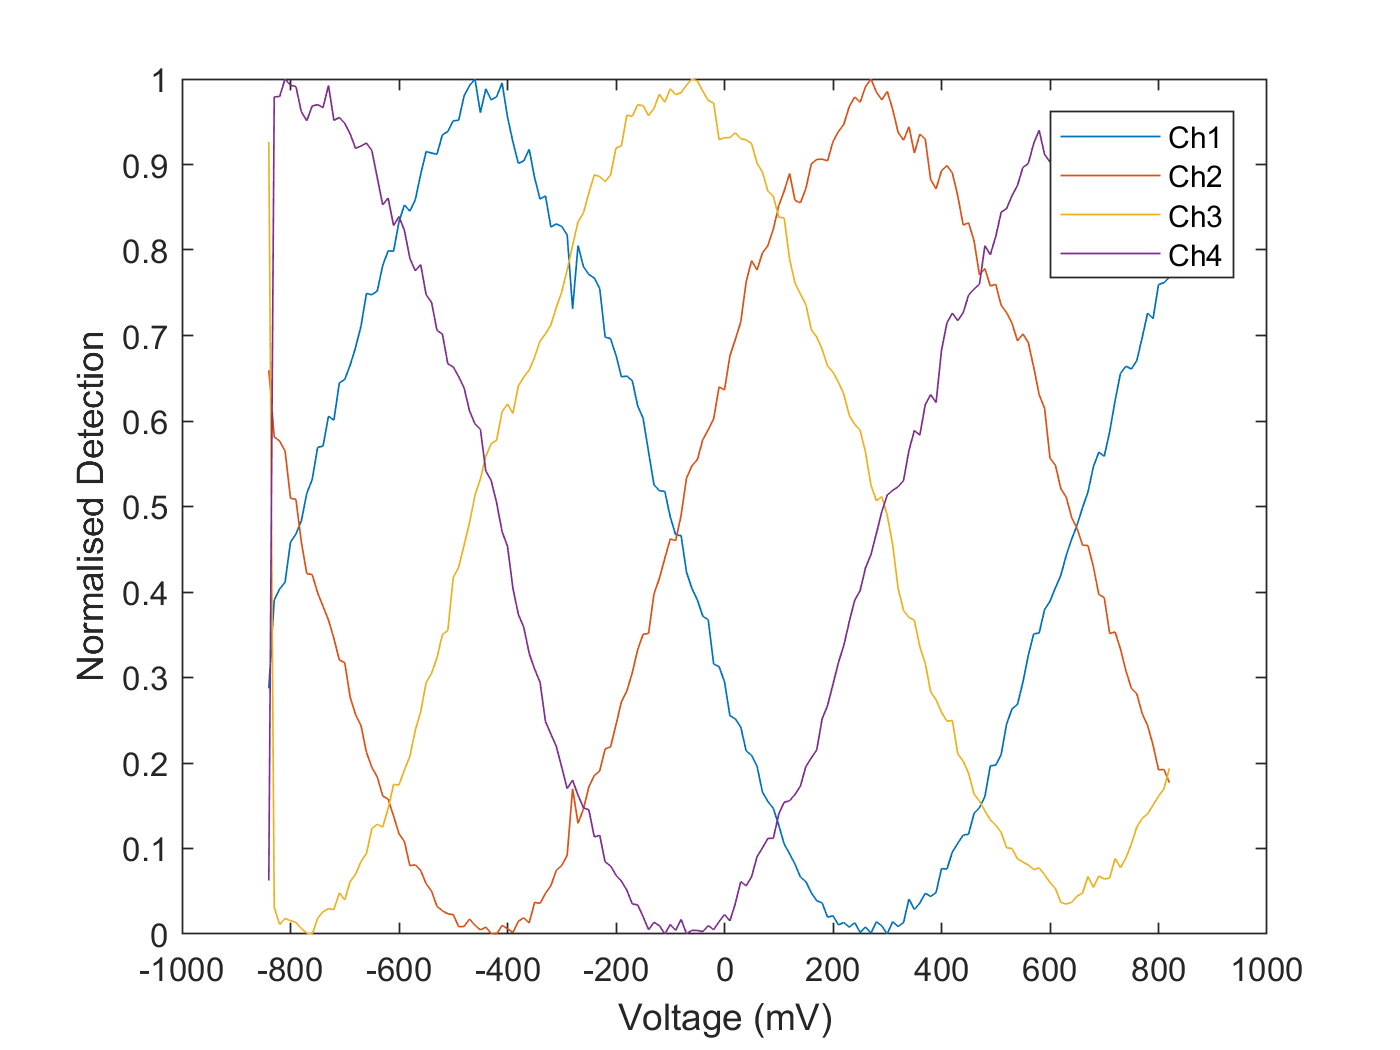
\includegraphics[height=0.33\textwidth,keepaspectratio]{NormalisedEOM}
\caption{\label{fig:NormalisedEOM}The normalised counts as a function of the voltage applied to the EOM amplifier for each detection channel. Channel: Ch1, Ch2, Ch3 and Ch4 measures counts of photons in the polarisation state: $\ket{R},\ket{L},\ket{V},$ and $\ket{H}$, respectively.}
\end{figure}

\begin{figure}[t]
\centering
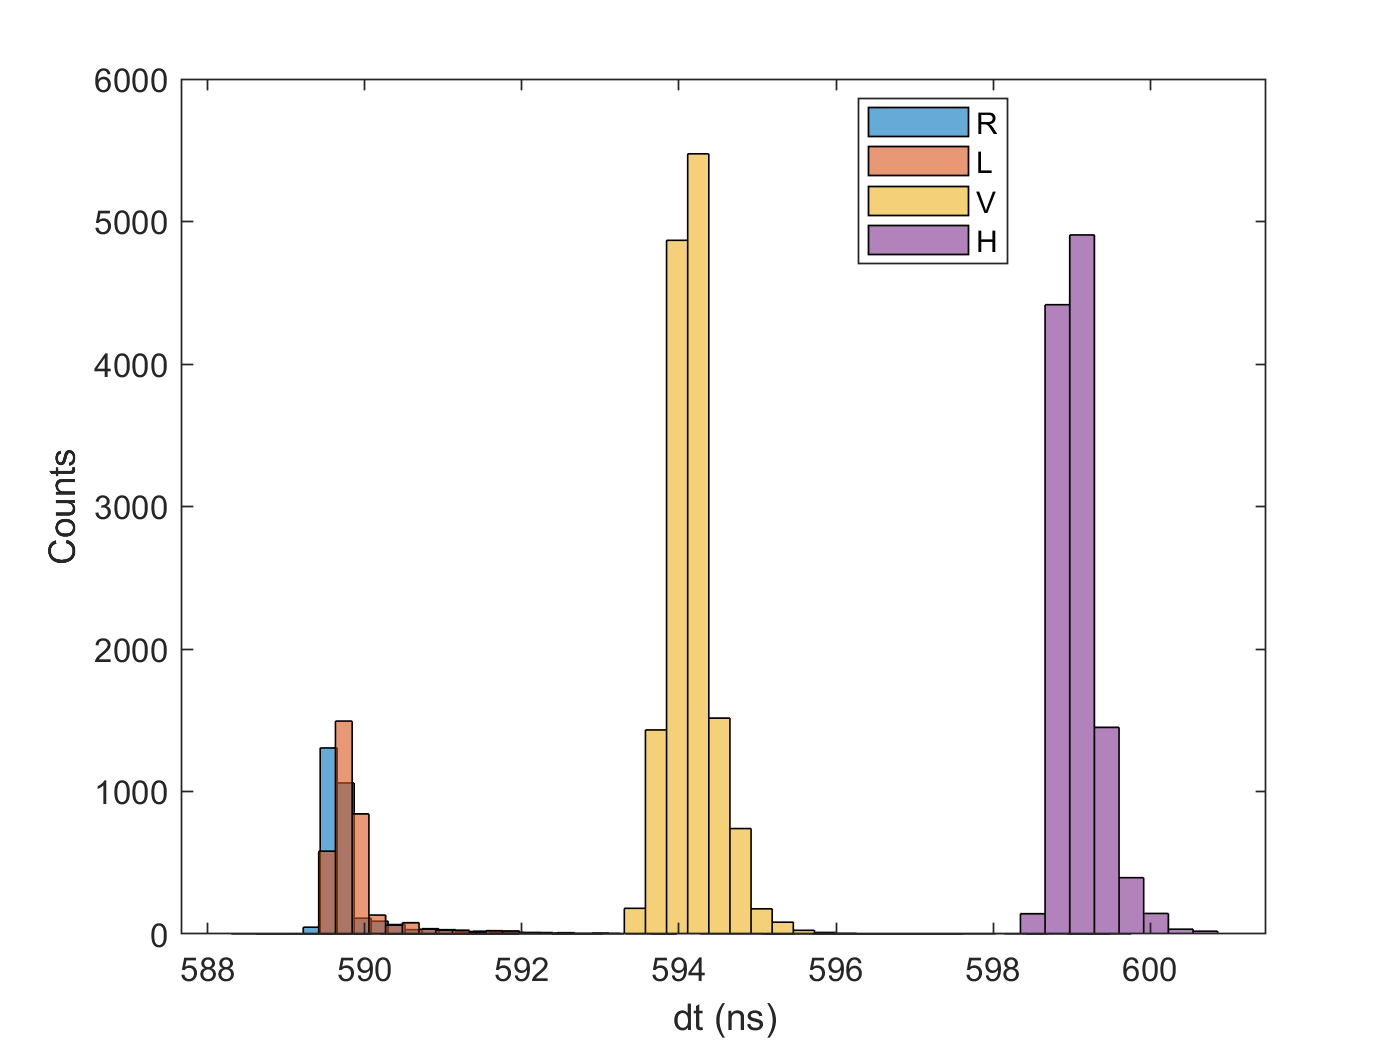
\includegraphics[height=0.33\textwidth,keepaspectratio]{histogramdt}
\caption{\label{fig:histogramdt}The time windowed histogram plot of the counts detected vs. the time between the trigger and the detection event.}
\end{figure} 

\begin{figure}[b]
\centering
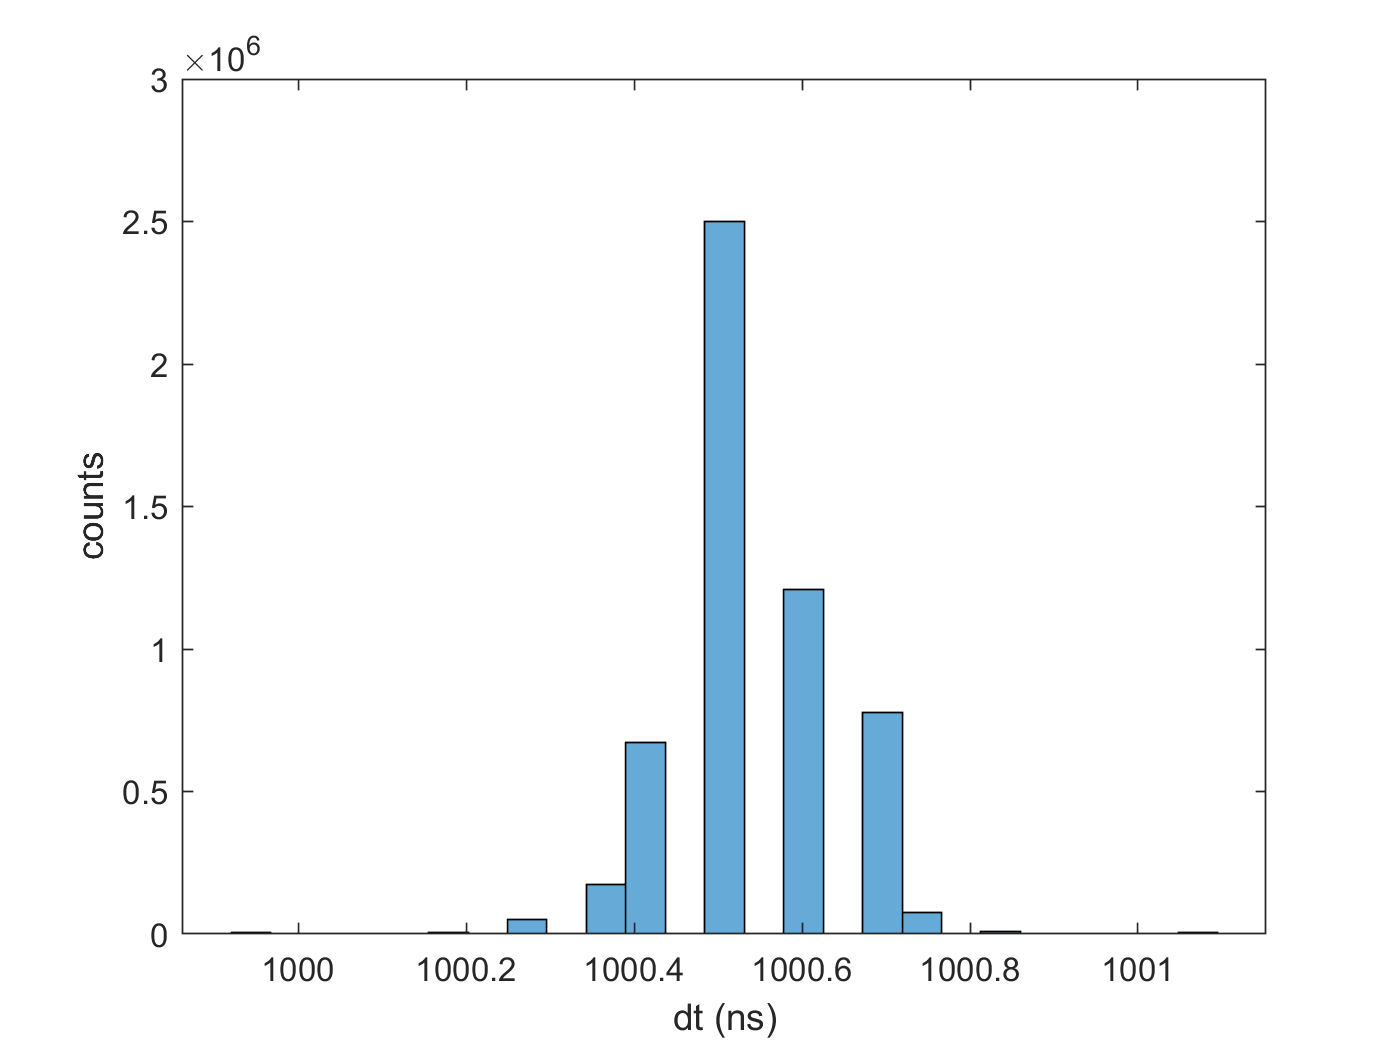
\includegraphics[height=0.33\textwidth,keepaspectratio]{triggerevents}
\caption{\label{fig:triggerevents}Counts vs. time between successive trigger detection events}
\end{figure}

The initial challenge of implementing this scheme is to align the optics shown in Fig. (\ref{fig:opticalsetup}). In particular the laser beam must be efficiently coupled into the fiber optics. To focus the beam into the fiber-couple the distance between the convex coupling lenses was altered in small increments. The DC voltage level was viewed on a oscilloscope by connecting the fiber output to a photon amplifier circuit. Due to the short time available to complete the BB84 experiment, analysis of previously measured data is presented. The ability to transfer a one-time pad with a sufficiency low bit error rate is investigated. 

Initially the small voltage applied $V_{app}$ to the EOM amplifier is swept over a range which will produce all polarisation states. The laser is operated as continuous wave (cw) and the photons are detected by APDs. Since the efficiency of each detector differs, the counts on each channel are rescaled using the data normalisation: $x{}'=(x-x_{max})/(x_{max}-x_{min})$. From the results shown in Fig. (\ref{fig:NormalisedEOM}), it is simple to determine which channel: Ch1, Ch2, Ch3 and Ch4 is connected to the APD which detects photons is the polarisation state: $\ket{R},\ket{L},\ket{V},$ and $\ket{H}$, respectively. The values of $V_{app}$ which correspond to the maximum value of each photon state are obtained to implement the optimum voltage sequence for the one-time pad distribution. 

The photon states sent by Alice, are detected by Bob where $dt$ refers to the difference in time between the trigger detection and the photon detection on a specific channel. The efficiency the APDs results in the difference in the counts across different channels as shown in Fig. (\ref{fig:histogramdt}) where the time window of $dt$ is $(5.88-6.01)\times10^{-7}$ s is chosen to reduce the number of dark counts recorded. The peak position for each histogram varies due to the difference in distance travelled by a single photon to reach each detector. The pulse width of the laser is approximated by calculating the full-width at half maximum (FWHM) from the standard deviation, $\sigma$ of $dt$ for each channel where FWHM = $2\sigma\sqrt{2\ln{2}}$. The average FWHM across the detection channels was 1.18 ns. This is several orders of magnitude larger than the quoted $\approx$ 80 ps pulse width that the laser is operated at. Additionally, the FWHM of for the $dt$ between consecutive trigger detections is calculated as 0.21 ns, this value thus gives the ultimate time resolution of the experiment. 

An estimation of the average photons per pulse is calculated as 0.06 where the individual detector efficiencies are taken as their quoted quantum efficiency. Since detectors are operated as single photon counters there is a dead time after detection reduces the ability to measure the approximately 5 $\%$ two photon occurrence events. Furthermore the dark count rates for the experiment APDs were estimated by initially finding a investigating histogram time binning of $dt$ such that there is a threshold value below which the approximation that any counts are tallied as dark counts is used. The dark count rate of Ch1 and Ch2 are 5.11 Hz and 6.94 Hz are compared to the quoted rate of < 2 Hz. The dark count rate of < 100 Hz is compared to the measured results of 141 Hz and 547 Hz for Ch3 and Ch4 respectively.       

\begin{figure}[t]
\centering
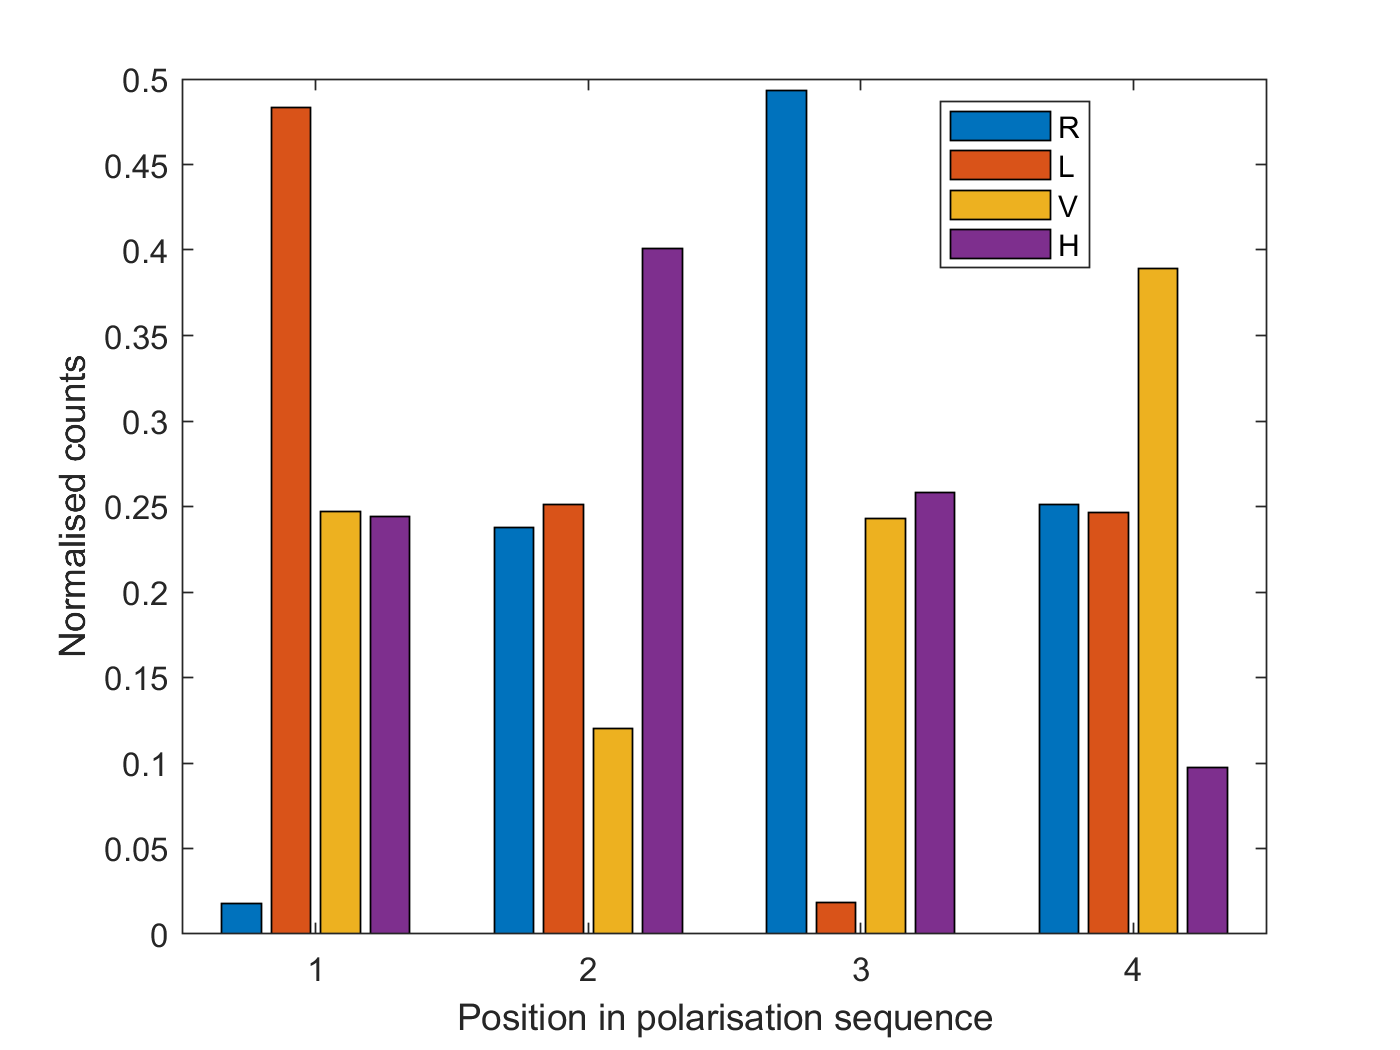
\includegraphics[height=0.33\textwidth,keepaspectratio]{countsvspolarisationstate}
\caption{\label{fig:countsvspolarisationstate}The normalised counts for each detection channel vs. the position in the state preparation sequence. Each colour on the chart corresponds to a different polarisation state detector.}
\end{figure} 

Since the sequence of the $V_{app}$ to the EOM amplifier is repetitive, the number of counts measured on each channel can be determined for the four possible positions in the $V_{app}$ sequence. Here the assumption is made that differences in detector efficiencies can be corrected for as the QKD scheme cannot operate if Bob is biased towards measuring certain states and not others. The normalisation of the counts on each polarisation detector is shown in Fig. (\ref{fig:countsvspolarisationstate}) where the blue bars will sum to 1 etc. From knowing the detectors for each polarisation state detector, the $V_{app}$ sequence prepares the photon states as: $\ket{L},\ket{H},\ket{R},$ and $\ket{V}$, respectively before repeating in this order. The 50 $\%$ probability the polarisation state is measured in the incorrect basis is displayed by the $\approx 1/2$ sum of normalised counts for these polarisation state detectors. This is due to the PBS effectively becoming a 50:50 BS if the photon is polarised in the wrong basis. Alice and Bob can remove these bits from the key string by communicating their prepared and the measurement basis. The QBER which refers to the rate at which errors occur when the data is transmitted is presented for the prepared $\ket{L}$ photon state in position 1. The result is calculated as $R_{1}/(R_{1}+L_{1})$= 3.51 $\%$. Similarly the QBER for the prepared $\ket{H}$, $\ket{R}$ and $\ket{V}$ are given as: 23.1 $\%$, 3.65 $\%$ and 19.9 $\%$, respectively. 




\section{\label{sec:level1}Discussion and Conclusion}
The significant difference between the estimated laser pulse width and quoted pulse width is suspected, at least in part, to be due to broadening of the FWHM due to the ultimate time resolution electronic detection being 0.21 ns and APD jitter time. The jitter time is the statistical fluctuation of the photon arrival time at the detector and the output of the electrical pulse \citep{Jani2007TimingCircuitry}. The jitter pulse is < 60 ps and $\approx$ 350 ps for the two APD types. The estimated 0.06 photons per pulse appears reasonable as BB84 schemes have been known to often be operated at $\bar{N}\approx0.1$ \citep{Fox2006QuantumIntroduction}. The dark count rate and the inability for the APD to complete two photon detection increases the uncertainty of the experimentally measured $\bar{N}$. The APD known dark count rates are lower than the experimentally measured values. This is not surprising due to the approximation used to gather dark count data. Additionally, if the fiber-coupling efficiency is not optimised the difference may also be due to photon state losses. 

Following the correction for differences in the APD efficiencies, the state detection results are shown in Fig. (\ref{fig:countsvspolarisationstate}). The expected characteristic results of the BB84 protocol for each generated EOM photon state is observed. Measurement in the correct basis results in the largest normalised count, whilst the approximately equal bars correspond photons being reflected to the opposite basis measurement arm. The QBER calculated determines that the scheme is not currently sufficiently secured. This is due to two of the error rates for two of the prepared states being about the 15$\%$ cut-off for completing secured quantum cryptography. Factors contributing to the increased QBER include dark counts and background light APD detection, imperfections of the EOM operation which can result in rotation of the plane of polarisation. The amplifier places limitations on the experiment where the trigger repetition rate determined from Fig. (\ref{fig:triggerevents}) is given as 1 MHz. The trigger rate is limited by the switching rate of the EOM amplifier. Additionally the voltage range being between $-V_{\pi}$ and $+V_{\pi}$, reduces the ability to generate light with only a polarisation component in the $\ket{H}$ direction. 

In conclusion, analysis of the data collected by a previous group enables useful insight into the current limiting factors of the experimental set-up. By addressing aspects such as improving the fiber the coupling efficiency, further shielding of the set-up from background light sources and optimising the voltage at which EOM produces the four light polarisation states could reduce the noise sources in the free-space optical set-up. Therefore, reducing the noise level of the imperfect quantum channel such that the QBER for the detection of each photon state is below < 15 $\%$ would allow the scheme to securely distribute a one-time pad.




\end{footnotesize}


\bibliographystyle{ieeetr}
\tiny
\bibliography{main}

\end{document}